\chapter{Modules}

  \begin{define}
    Let $R$ be a ring. A \bt{left $\bs{R}$-module} is an abelian group
    $(M,+)$ endowed with an action of $R$, i.e. a map $R\times M \to M$,
    usually denoted $(r,m)\mapsto rm$, such that
    \begin{enumerate}
      \item $(r + r')m = rm+r'm$, $r(m+m') = rm+rm'$
      \item $1m = m$
      \item $(rs)m = r(sm)$
    \end{enumerate}
  \end{define}
  This is the same data as a ring homomorphism $R \to \End_\ZZ M$.

  Examples:
  \begin{enumerate}
    \item $\{0\}$. $r\cdot 0 = 0$
    \item $\sub{R}{R}$ where $r\cdot m = rm$.
    \item If $M$ is a left $R$-module, it becomes a right $R^{\op}$-module by
      $mr^o = rm$.
  \end{enumerate}

  \begin{prop}
    A module over a field $k$ is a $k$-vector space.
  \end{prop}

  \begin{define}
    A subgroup $N$ of a left $R$-module $M$ is a \bt{submodule} if $rn\in N$
    for all $r\in R$ and $n\in N$.
  \end{define}

  The submodules of $\sub{R}{R}$ are the left ideals of $R$.

  \begin{define}
    A non-zero left $R$-module $M$ is \bt{simple} if its only submodules are
    $\{0\}$ and $M$ itself.
  \end{define}

  \begin{define}
    If $M$ and $N$ are left $R$-modules, a map $f:M\to N$ is a
    \bt{homomorphism} of left $R$-modules if it is a group homomorphism
    and $f(rm) = rf(m)$ for all $r\in R$ and $m\in M$.
  \end{define}

  \begin{define}
    A homomorphism $f$ of $R$-modules is an \bt{isomorphism} if it is
    bijective.
  \end{define}
  The bijectivity allows us to define $f^{-1}$ and $f^{-1}$ is an $R$-module
  homomorphism.

  \begin{define}
    If $N$ is a submodule of $M$, then $M/N$ becomes a left $R$-module via
    \[ r(m + N) = rm + N, \]
    we call this a \bt{quotient module}.
  \end{define}
  Observe that if $m-m'\in N$, then $rm - rm'\in N$ for all $r\in R$. So
  $r(m+N)$ is well-defined.

  More module examples:
  \begin{enumerate}
    \item $R/I$ where $I$ is a left ideal of $R$.
    \item If $M$ and $N$ are left $R$-modules, their direct sum
      \[ M\oplus N = \{(m,n): m \in M, n\in N\} \]
      is a left $R$-module via $r(m,n) = (rm,rn)$.
    \item free $R$-modules of finite rank: these are
      \[ R^n = \underbrace{R \oplus \cdots \oplus R}_{n\text{ times}}. \]
      If $I_1,\ldots,I_n$ are left ideals of $R$, then
      $I_1\oplus \cdots \oplus I_n$ is a submodule of $R^n$.
    \item Let $R$ be the ring of differential operators with $\CC$-valued
      polynomials as coefficients. Then $\CC[x]$ is a left $R$-module via
      $D \cdot f = D(f)$. e.g. let $D=(1-x^2)\frac{d^2}{dx^2}+2x\frac{d}{dx}$
      and $f(x) = 2x-1$, then $D(f) = 4x$.
  \end{enumerate}

  \begin{lemma}
    If $f:M\to N$ is an $R$-module homomorphism, then $\ker f$ is a submodule
    of $M$, the image of $f$ is a submodule of $N$ and $M/\ker f \cong \im f$
    as $R$-modules via $m+\ker f \mapsto f(m)$.
  \end{lemma}

  \begin{define}
    If $M$ is a left $R$-module, we write $\End_R{M} = \{f:M\to M\}$, this is
    called the \bt{Endomorphism Ring} of $M$.
  \end{define}

  \begin{lemma}[Schur's Lemma]
    If $M$ is a simple $R$-module, then $\End_R{M}$ is a division ring.
  \end{lemma}

  \begin{prop}
    If $M$ is a left $R$-module, there is a ring homomorphism
    $\psi:Z(R)\to\End_R{M}$ given by $\psi(z)(m)=zm$.
  \end{prop}

  \begin{cor}
    If $R$ is a $k$-algebra and $M$ a left $R$-module, then there is a
    homomorphism $k \to\End_R{M}$.
  \end{cor}

  \begin{thm}[Dixmier's Theorem]
    If $R$ is a $\CC$-algebra of countable dimension, and $M$ is a simple
    $R$-module, then the canonical map $\psi:\CC \to \End_R{M}$ is an
    isomorphism.
  \end{thm}

  \begin{lemma}
    If $I$ is a left ideal in $R$ and $I\neq R$, then there is a maximal
    left ideal that contains $I$.
  \end{lemma}
  \begin{proof}
    Let $\Ac$ be the set of left ideals that contain $I$ and are not $R$, then
    there is a sequence $I_1 \subset I_2 \subset \cdots$ of $I_j\in \Ac$. But
    $\bigcup I_j$ is a left ideal, which is maximal, containing $I$.
  \end{proof}

  \begin{prop}\label{mod:max_ind}
    If $R$ has a unique maximal left ideal, $\sub{R}{R}$ is indecomposable.
  \end{prop}
  \begin{proof}
    Let $J$ be the unique maximal left ideal, then if $R = L+N$ for some left
    ideals $L$ and $N$, and $L\neq R$, then $L\subseteq J$. Hence
    $N\not\subseteq J$, and so $N=R$, which implies that  if $L\neq 0$,
    $L\cap N \neq 0$.
  \end{proof}

  \begin{prop}
    Let $R=k[x_1,\ldots,x_n]$ and let $m=(x_1,\ldots,x_n)$. If $I\supseteq m^d$
    for some $d$, then $R/I$ is an indecomposable $R$-module (because it has a
    unique maximal ideal, namely $m/I$).
  \end{prop}
  \begin{proof}
    Every maximal ideal of $R/I$ is of the form $n/I$ for some maximal ideal
    $n$ of $R$ containing $I$. Now $R/n$ is a simple $R$-module and
    $I\cdot(R/n) = (I+n)/n = n/n = 0$, but $m^d \subseteq I$, so $m^d(R/n)=0$.
    If $S$ is a simple left $R$-module and $J$ is any left ideal of $R$, then
    $JS$ is a submodule of $S$ so either $JS = 0$ or $JS = S$. However, if
    $JS=S$, then $J^dS = S$ for all $d$, so $m(R/n) = 0$. But
    $m(R/n) = (m+n)/n$ so $m\subseteq n$, which implies $m = n$ since $m$ and
    $n$ are both maximal ideals. By Proposition \ref{mod:max_ind}, $R/I$ is
    an indecomposable $R/I$-module and hence an indecomposable $R$-module.
  \end{proof}

  \begin{define}
    A \bt{basis} for a module $M$ is a subset $S \subseteq M$ such
    that every element $m\in M$ can be written in a unique way as
    \[m = \sum_{b\in S} rb, \]
    for a unique set of $r \in R$, only finitely many of which are non-zero.
  \end{define}

  \begin{define}
    A left $R$-module $F$ is \bt{free} if it has a basis.
  \end{define}

  Example: If $X$ is a finite set $R^X = \{\text{functions } X\to R\}$ is
  a free module via $(rf)(x) = rf(x)$ for all $r\in R,f\in R^X,x\in X$, and
  $R^X \cong \underbrace{R\oplus\cdots\oplus R}{|X|\text{ times}} = R^{|X|}$.

  \begin{define}
    We say $R$ has the \bt{invariant basis number} property if all bases for
    each free module have the same number of elements.
  \end{define}

  $\Mod(R)$ is the category of left $R$-modules

  Let $k$ be a field, then $\Mod(k)$ are vector spaces.
  \begin{itemize}
    \item Unique simple object up to isomophism, $k$.
    \item Every object in $\Mod(k)$ is isomorphic to a direct sum of copies of
      $k$.
    \item $\Hom(k,k) \cong k$.
  \end{itemize}

  Now let $R = M_2(k)$, and consider $\Mod(R)$.
  \begin{itemize}
    \item It has a unique simple object up to isomorphism, namely
    \[ K = \begin{bmatrix} k \\ k \end{bmatrix} = \left\{\begin{bmatrix} a \\ b\end{bmatrix} : a,b\in k\right\} \]
    \item Ever $R$-module is isomorphic to direct sum of copies of $K$.
    \item $\Hom_R(K,K) \cong k$.
  \end{itemize}

  \begin{prop}
    $\Mod(k)$ is equivalent to $\Mod(R)$
  \end{prop}
  \begin{proof}
    $\Mod(K) \to \Mod(R)$, where $V \mapsto \Hom_k(k^2,V) \ni f$, then
    $(rf)(u) = f(ru)$. The free $k$-module $k\mapsto \Hom_k(k^2,k)$ is two
    dimensional. Every $f$-dimensional free $M_2(k)$ has dimension a multiple
    of four. The equivalence $\Mod(k)\to \Mod(M_2(k))$ does not send free
    $k$-modules to free $M_2(k)$-modules.
  \end{proof}

  So freeness is not a categorical property.

  The best things in life are $\cancel{\text{free}}$ projective. (Free modules
  are projective but not conversely in general.)

\section{Exact Sequences}

  \begin{define}
    Fix $R$. A sequence of $R$-modules and homomorphisms
    \[ \cdots \to A_n \stackrel{f_n}{\to} A_{n+1} \stackrel{f_{n+1}}{\to} A_{n+2} \to \cdots \]
    is \bt{exact} if $\ker{f_{n+1}} = \im{f_n}$ for all $n$.
  \end{define}
  \begin{define}
    A \bt{short exact sequence} is an exact sequence of the form
    \[ 0 \to L \to M \to N \to 0. \]
  \end{define}

  \begin{lemma}
    A sequence
    \[ 0 \to L \stackrel{f}{\to} M \stackrel{g}{\to} N \to 0 \]
    is exact if and only if
    \begin{enumerate}
      \item $f$ is injective
      \item $\ker{g} = \im{f}$
      \item $g$ is surjective
    \end{enumerate}
  \end{lemma}

  In this situation $N \cong M/f(L)$ via
  \[ [m+f(L)] \mapsto g(m). \]

  If $L$ is a submodule of a module $M$, then there is a short exact sequence
  \[ 0 \to L \to M \to M/L \to 0, \]
  where $l\mapsto l$ and $m\mapsto [m+L]$.

  Every short exact sequence in $\Mod(R)$ is isomorphic to a short exact
  sequence to the form
  \[ 0 \to L \to M \to M/L \to 0. \]

  \begin{define}
    Let $R$ and $S$ be rings, an \bt{$\bs{R}$-$\bs{S}$-bimodule} is a left $R$-module
    with a right $S$-module such that
    \[ r(ms) = (rm)s \]
    for all $r\in R$, $s\in S$, and $m\in M$.
  \end{define}

  \begin{lemma}
    Let $M$ be a right $S$-module, then $M$ is an $\End_S{M}-S$-bimodule.
  \end{lemma}
  \begin{proof}
    Make $M$ a left $\End_S{M}$-module by
    \[ fm = f(m); \]
    this makes $M$ a left $\End_S{M}$-module and $(fm)s = f(m)s = f(ms)$.
  \end{proof}

  \begin{prop}
    Let $M$ be an $R$-$S$-bimodule and $N$ a $T-U$-bimodule. Then
    $\Hom_\ZZ(M,N)$ is a left $T$-module, a left $S$-module, a right
    $R$-module, a right $U$-module, a $T$-$R$-bimodule, a $T$-$U$-bimodule, a
    $S$-$R$-bimodule, and a $S$-$R$-bimodule.
  \end{prop}
  \begin{proof}
    If $f\in \Hom_\ZZ(M,N)$ then
    \begin{align*}
      (tfr)(m) &= tf(rm) \\
      (sfu)(m) &= f(ms)u.
    \end{align*}
  \end{proof}

  Special case: $\sub{R}{M}_S, \sub{T}{N}_U$, then $\Hom_R(M,N)$ is an
  $S$-$U$-bimodule via $(sfu)(m) = f(ms)u$. Additionally $\Hom_R(M,R)$ is a
  $S$-$R$-bimodule, in particular it is a right $R$-module. The rule
  $\sub{R}{M} \to \Hom_R(M,R)$ is a contravariant functor from
  $\Mod_l R \to \Mod_r R$.

  \begin{thm}[Dual Basis lemma]
    Let $P$ be a left $R$-module, then $P$ is projective
    if and only if there are sets $\{p_i:i\in I\}\subset P$ and
    $\{\vphi_i: i\in I\} \subset \Hom_R(P,R)$ such that
    \begin{itemize}
      \item if $p\in P$, $\vphi_i(p)\neq 0$
      \item if $p\in P$, then $p = \sum_{i\in I}\vphi_i(p)p_i$.
    \end{itemize}
  \end{thm}
  \begin{proof}
    Assume that $P$ is projective, so there exists $Q$ such that $P\oplus Q$
    is free. Let $\{e_i:i\in I\}$ be a basis for $P\oplus Q$, and write
    $e_i = p_i+q_i=(p_i,q_i)$ with $p_i \in P$ and $q_i \in Q$. If
    $x = \sum_{i\in I}r_ie_i$, then let $\phi_i:P\oplus Q\to R$ be
    $\phi_i(x) = r_i$, and let $\vphi_i:P\to R$ be the restriction of $\phi_i$
    to $P\subseteq P\oplus Q$. Let $p\in P$, and write
    \[ p=\sum r_ie_i=\sum \vphi_i(p)e_i=\sum\vphi_i(p)p_i + \sum \vphi_i(p)q_i, \]
    then $\sum \vphi_i(p)q_i \in Q\cap P = 0$, so $p = \sum \vphi_i(p)p_i$.

    Now let $F$ be the free left $R$-module on a basis indexed by $I$, i.e.
    $\{ b_i: i\in I\}$. Define $\theta:F\to P$ by $\theta(b_i) = p_i$. Note
    that $\theta$ is a surjective homomorphism of left $R$-modules, so define
    $\mu:P\to F$ by $\mu(p) = \sum \vphi_i(p)b_i$. This is an $R$-module
    homomorphism and
    \[ (\theta\circ \mu)(p) = \theta\left(\sum \vphi_i(p)b_i\right) = \sum\vphi_i(p)\theta(b_i) = \sum\vphi_i(p)p_i = p,\]
    so $\theta\circ \mu = \Id_P$. Hence the sequence
    $0\to\ker\theta\to F\to P\to 0$ splits, so $F\cong P\oplus \ker\theta$,
    and hence $P$ is projective.
  \end{proof}

  \begin{thm}[Structure Theorem for Modules over Principle Ideal Domains]
    If $R$ is a principle ideal domain and $M$ is a finitely generated
    $R$-module, then
    \[ M\cong R^n\oplus \frac{R}{m_1^{t_1}}\oplus \cdots \oplus \frac{R}{m_k^{t_k}} \]
    for some integers $n\geq 0$, $k\geq 0$, and $t_1,\ldots,t_k>0$ and some
    maximal ideals $m_1,\ldots m_k$.
  \end{thm}

  \begin{cor}[Structure Theorem for Finitely Abelian Groups]
    If $G$ is finitely abelian group, then
    \[ G \cong \ZZ^n \oplus \frac{\ZZ}{p_1^{t_1}\ZZ} \oplus \cdots \oplus \frac{\ZZ}{p_k^{t_k}\ZZ} \]
    for some integers $n\geq 0$, $k\geq 0$, and $t_1,\ldots,t_k>0$ and some
    primes $p_1,\ldots,p_k$.
  \end{cor}

\section{Quivers}

  \begin{define}
    A \bt{quiver} is a finite directed graph i.e. finite number of vertices
    and arrows.
  \end{define}
  Often write $Q=(Q_0,Q_1)$, where $Q_0$ is a set of vertices and $Q_1$ is a
  set of arrows.

  \begin{define}
    A representation of a quiver $Q$ (for a fixed field $k$) is a collection of
    vector spaces $V_i$, $i\in Q_0$ and linear maps
    $\alpha_a:V_{s(a)} \to V_{t(a)}$, $a\in Q_1$, where $s(a)$ is the base of
    $a$ and $t(a)$ is the tip of $a$.
  \end{define}

  \begin{define}
    Homomorphisms between representations are maps
    \[ \Phi:(V_i, \alpha_a) \to (U_i, \beta_a),\]
    is a collection of linear maps $\Phi_i:V_i\to U_i$, such that the following
    commutes
    \begin{center}
    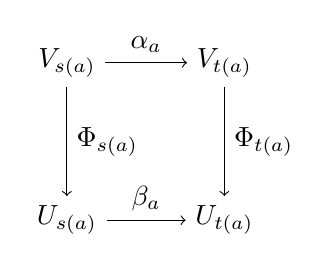
\begin{tikzpicture}
      \draw node (00) {$V_{s(a)}$};
      \draw (2,0) node (10) {$V_{t(a)}$};
      \draw (0,-2) node (01) {$U_{s(a)}$};
      \draw (2,-2) node (11) {$U_{t(a)}$};
      \draw[->] (00) -> node[above] {$\alpha_a$} (10);
      \draw[->] (01) -> node[above] {$\beta_a$} (11);
      \draw[->] (00) -> node[right] {$\Phi_{s(a)}$} (01);
      \draw[->] (10) -> node[right] {$\Phi_{t(a)}$} (11);
    \end{tikzpicture}
  \end{center}
  \end{define}

  \begin{thm}
    There is an equivalence of categories
    \[ \Rep(Q) \equiv \Mod(kQ) \]
    where $kQ$ is the path algebra of $Q$, i.e. $kQ$ is the vector space with
    basis $\{\text{paths in }Q\}$.
  \end{thm}
